\documentclass[11pt,a4paper]{article}

\usepackage[margin=2.4cm]{geometry}
\usepackage{lmodern}
\usepackage[T1]{fontenc}
\usepackage[utf8]{inputenc}
\usepackage{amsmath,amssymb,amsthm,bm}
\usepackage{booktabs,array,tabularx}
\usepackage{microtype}
\usepackage{setspace}
\usepackage{xcolor}
\usepackage{caption}
\usepackage{placeins}
\usepackage{tikz}
\usetikzlibrary{arrows.meta,positioning,calc}
\usepackage{pgfplots}
\usepgfplotslibrary{groupplots}
\pgfplotsset{compat=1.18}
\usepackage[hidelinks]{hyperref}

\definecolor{ink}{HTML}{1B4F72}
\definecolor{soft}{HTML}{EAF0F4}
\definecolor{teal}{HTML}{16837A}
\definecolor{amber}{HTML}{C56A00}
\definecolor{crit}{HTML}{A13D35}
\definecolor{mid}{HTML}{65727C}
\hypersetup{colorlinks=true,linkcolor=ink,citecolor=ink,urlcolor=ink}

\newcommand{\E}{\mathbb{E}}
\newcommand{\Var}{\mathrm{Var}}
\newcommand{\Cov}{\mathrm{Cov}}
\newcommand{\Corr}{\mathrm{Corr}}
\newcommand{\doi}[1]{\href{https://doi.org/#1}{doi:\allowbreak\texttt{#1}}}
\newcommand{\code}[1]{\texttt{#1}}
\newcommand{\pkg}[1]{\texttt{#1}}
\newcommand{\Rtwo}{\(R^2\)}
\emergencystretch=2em
\newcolumntype{L}[1]{>{\raggedright\arraybackslash}p{#1}}
\newcolumntype{Y}{>{\raggedright\arraybackslash}X}

% Generated by report/generate_evidence.py; do not edit.
\newcommand{\ReportPackageVersion}{0.3.4.dev3}
\newcommand{\ReportSourceRevision}{7eb369be5393}
\newcommand{\ReportInputDigest}{0cd51b755406ef69970d9faa572228eaba7a5200179241d402ba47e900afa43c}
\newcommand{\ReportInputDigestDisplay}{\texttt{0cd51b75\allowbreak{}5406ef69\allowbreak{}970d9faa\allowbreak{}572228ea\allowbreak{}ba7a5200\allowbreak{}179241d4\allowbreak{}02ba47e9\allowbreak{}00afa43c}}
\newcommand{\ReportTestCount}{461}
\newcommand{\ReportPythonVersion}{3.14.6}
\newcommand{\ReportNumpyVersion}{2.4.6}
\newcommand{\ReportScikitLearnVersion}{1.9.0}
\newcommand{\ReportPytestVersion}{9.1.1}
\newcommand{\ReportLdpredThreeVersion}{0.7.21.dev0}
\newcommand{\ReportFitReplicates}{240}
\newcommand{\ReportFitWins}{240}
\newcommand{\ReportFitUpliftMin}{0.0660}
\newcommand{\ReportFitUpliftMax}{0.2307}
\newcommand{\ReportFitGapClosedMinPct}{83.4}
\newcommand{\ReportFitGapClosedMaxPct}{99.2}
\newcommand{\ReportFitCvMinusHoldout}{-0.00230}
\newcommand{\ReportNullPasses}{11}
\newcommand{\ReportNullReplicates}{60}
\newcommand{\ReportSumstatBetaCorrelation}{0.999858}
\newcommand{\ReportSumstatRtwoMin}{0.4973}
\newcommand{\ReportSumstatRtwoMax}{0.4983}
\newcommand{\ReportPumasGaussianErrorPct}{3.77}
\newcommand{\ReportPumasBinaryErrorPct}{10.99}
\newcommand{\ReportLdTrueDropNfifty}{0.01795}
\newcommand{\ReportLdInflationNfifty}{0.04446}
\newcommand{\ReportLdInflationNfiftyPct}{26.4}
\newcommand{\ReportOverlapMultiRatioTen}{2.03}
\newcommand{\ReportOverlapSingleRatioTen}{4.89}
\newcommand{\ReportOverlapMultiRatioTwentyFive}{3.98}
\newcommand{\ReportOverlapSingleRatioTwentyFive}{14.73}
\newcommand{\ReportOverlapDetectedNonnull}{16}
\newcommand{\ReportOverlapNonnullReplicates}{16}
\newcommand{\ReportOverlapDetectedNull}{0}
\newcommand{\ReportOverlapNullReplicates}{8}
\newcommand{\ReportRealMetaExpectedRtwo}{0.17729}
\newcommand{\ReportRealMetaDecorrelatedRtwo}{0.002261}

\hypersetup{pdfsubject={multipgs-input-sha256=\ReportInputDigest;multipgs-version=\ReportPackageVersion}}

\title{%
  \vspace{-1.4em}
  {\large Notes}\\[0.4em]
  {\LARGE\bfseries Combining polygenic scores}\\[0.15em]
  {\large Selection index, three information routes,\\
   and evidence in \texttt{multipgs}}}
\author{Bjarni J\'ohann Vilhj\'almsson\\[0.35em]
  {\small\texttt{https://github.com/bvilhjal/multipgs}\quad$\cdot$\quad
   v\ReportPackageVersion}}
\date{13 August 2026}

\begin{document}
\maketitle
\thispagestyle{plain}

\begin{abstract}
\noindent
A linear combination of existing polygenic scores is a selection
index. Write \(Z\) for the vector of standardised component scores
in a target population, \(\rho_k=\Corr(Z_k,g_f)\) for the
correlation of score \(k\) with the focal genetic value, and \(C\)
for the correlation matrix of \(Z\). The squared genetic-value
correlation of a weight vector \(w\) is
\((w^{\mathsf T}\rho)^2/(w^{\mathsf T}Cw)\). When \(C\) is
positive definite the optimum is \(w_\star\propto C^{-1}\rho\).
For the focal score and one auxiliary score the exact increment is
\(\Delta R^2=r_G^2R_k^2(1-R_f^2)^2/(1-r_G^2R_f^2R_k^2)\). Absolute
gain therefore falls as the square of the information still
missing from the focal score.

The package implements three routes to an approximate index:
penalised stacking from a phenotyped target cohort, the same
Gaussian objective from score-space GWAS moments, and a
training-free same-trait rule. They solve different information
problems. In 240 held-out simulations where the genetic value
lies in the score span, the individual stack beat the
training-selected best single score in every replicate and closed
83.4--99.2\% of the oracle gap. Exact individual moments recover
the same coefficients (mean correlation \(0.999624\)). A small LD
reference and known discovery overlap inflate reported \Rtwo{}
more than they degrade the fitted predictor. Decorrelation is
exact under the intended \(\rho\) and collapses when that vector
is replaced by a Daetwyler proxy.

These results establish numerical identities and controlled
estimator behaviour. They do not establish clinical utility,
ancestry portability, or real-world comparative superiority.
\end{abstract}

\vspace{0.4em}
\noindent
The intended reader already uses polygenic scores, GWAS summary
statistics, and the distinction between a discovery sample and a
target cohort. These notes do not re-derive single-trait PGS
construction. They fix the combination estimand --- many-trait
score stacking, not a same-trait method ensemble --- the
selection-index algebra, the three information routes, and which
simulation claims survive their design.

\tableofcontents
\vspace{0.6em}

%----------------------------------------------------------------------
\section{Introduction}
\label{sec:intro}

A polygenic score (PGS) is a linear predictor of trait value
built from a genome-wide association study (GWAS)
\cite{dudbridge2013,choi2020}. Its accuracy is bounded by
discovery sample size, SNP heritability, and the effective number
of independent effects \cite{daetwyler2008,dudbridge2013}. Many
traits of interest have smaller discovery GWAS than genetically
correlated phenotypes. The usual response is to borrow strength.

The same linear-index algebra is used on three different
panels. Table~\ref{tab:neighbours} names them.

Family~(a) combines \emph{before} scoring: a multivariate model
reweights variant-level summaries, as in MTAG or wMT-SBLUP
\cite{turley2018,maier2018}. Family~(b) builds one score per
source and combines the scores. That family still splits. One
branch ensembles several constructions of the \emph{same} trait
--- methods, ancestries, or GWAS --- as in metaGRS, PRSmix,
PUMAS-ensemble, and MIXPRS
\cite{inouye2018,truong2024,zhao2024,xu2026}. The other branch
stacks scores of \emph{many traits}, as in Krapohl, Albi\~nana,
and PRSmix+ \cite{krapohl2018,albinana2023,truong2024,lambert2021}.
Family~(c) derives the combination weights from metadata rather
than from a target phenotype \cite{maier2018,smith1936,hazel1943}.

MIXPRS combines JointPRS-auto and SDPRX for one trait across
ancestries. Its weights are non-negative least squares on a
data-fission split of the target GWAS; SNP pruning plus an
identity residual is used so that a mismatched LD reference does
not correlate the pseudo-training and pseudo-tuning residuals
\cite{xu2026}. That is a same-trait method ensemble. It is not
multi-PGS. The MIXPRS discussion lists PRS for related traits as
future work; that is the problem this package addresses.

\begin{table}[ht]
\centering
\caption{Neighbouring combination methods, distinguished by the
  object in the linear index. \pkg{multipgs} implements the last
  two rows.}
\label{tab:neighbours}
\small
\begin{tabularx}{\linewidth}{@{}L{28mm}Y L{42mm}@{}}
\toprule
\textbf{Object} & \textbf{Examples} & \textbf{This package} \\
\midrule
Variant effects of several traits, before scoring &
MTAG, wMT-SBLUP & Not implemented \\
Same-trait methods or ancestries &
MIXPRS, PUMAS-ensemble, metaGRS, PRSmix &
\code{meta\_pgs} is the metadata-weight case only;
MIXPRS itself is not implemented \\
Scores of many traits &
Albi\~nana, Krapohl, PRSmix+ &
\code{multi\_pgs\_fit}, \code{multi\_pgs\_sumstats} \\
\bottomrule
\end{tabularx}
\end{table}

The published Multi-PGS analysis trained standardised scores with
unpenalised covariates and reported fivefold out-of-sample
assessment \cite{albinana2023}. \pkg{multipgs} implements that
broad estimator, but it is not a reproduction of the paper's
procedure. The package standardises inside training folds,
selects and averages coefficients by cross-model selection and
averaging (CMSA) \cite{prive2019}, adds a nested fallback gate,
supports a score-space summary-statistic objective, and reports
an unnormalised incremental \Rtwo{}. Those differences are
identifying, not cosmetic.

The rest of the note is the estimand (\S\ref{sec:estimand}), the
selection-index model (\S\ref{sec:index}), the three routes
(\S\ref{sec:routes}), deployment and metrics
(\S\ref{sec:deploy}), the simulation evidence
(\S\ref{sec:evidence}), the unit-test contracts
(\S\ref{sec:tests}), and the interpretation limits
(\S\ref{sec:limits}).

%----------------------------------------------------------------------
\section{Estimand}
\label{sec:estimand}

Write \(S_{ik}\) for the raw allele-weighted score of individual
\(i\) on component \(k=1,\ldots,K\), and write
\begin{equation}
  Z_{ik}=\frac{S_{ik}-\mu_k}{\sigma_k},
  \qquad
  \beta_k=\frac{\theta_k}{\sigma_k},
  \label{eq:standardization}
\end{equation}
for the training-standardised score and the corresponding
raw-scale coefficient. Penalisation is defined on \(\theta\).
Confusing these coordinates changes the meaning of every penalty
factor. Notation used throughout is collected in
Table~\ref{tab:notation}.

The package does not discover variants or estimate GWAS effects.
It starts from component weights that already exist. The object
it returns is a single deployable variant-weight vector
\begin{equation}
  \widetilde w_j=\sum_{k=1}^{K}w_{jk}\beta_k,
  \label{eq:combined-weights}
\end{equation}
where \(w_{jk}\) is the component weight of variant \(j\) in
score \(k\). Assessment of \(\widetilde w\) must use data
untouched by component discovery, combination fitting, and
tuning. That is the scientific claim. Everything else is a route
to \(\beta\).

Three estimands share that deployable object and are otherwise
distinct.

\paragraph{Learned combination.}
Given a phenotyped target sample, or given score-space moments
that stand in for one, the target is a penalised predictive
coefficient \(\theta\) for the observed phenotype \(y\) in the
span of the supplied scores. The coefficients are not genetic
correlations, not mediation weights, and not a feature-selection
discovery.

\paragraph{Same-trait index.}
When every component estimates the same genetic value, the
target is the selection-index direction \(w\propto C^{-1}\rho\)
under a stated model for \(\rho\). Metadata enter only through
that model.

\paragraph{What is not an estimand here.}
Absolute risk, a calibrated probability, an ancestry-adjusted
mean, or a causal decomposition of the panel. A
method-by-ancestry ensemble of one trait, as in MIXPRS
\cite{xu2026}, is a neighbouring estimand and is not implemented.
A high ranking metric is not any of those things.

\begin{table}[ht]
\centering
\caption{Notation used consistently in this report.}
\label{tab:notation}
\small
\begin{tabularx}{\linewidth}{@{}L{22mm}Y@{}}
\toprule
\textbf{Symbol} & \textbf{Meaning} \\
\midrule
\(n\), \(K\) & number of target individuals and number of
component scores \\
\(S\), \(Z\) & raw and training-standardised score matrices \\
\(\theta\), \(\beta\) & standardised-score and raw-score
coefficients, related by \eqref{eq:standardization} \\
\(g_k\), \(g_f\) & standardised additive genetic values for
component trait \(k\) and focal trait \(f\) \\
\(R_k\) & \(\Corr(Z_k,g_k)\), genetic-value accuracy of score
\(k\) for its own trait \\
\(r_G(k,\ell)\) & target-population genetic correlation between
traits \(k\) and \(\ell\) \\
\(\rho\) & target-population vector with
\(\rho_k=\Corr(Z_k,g_f)\) \\
\(C\) & correlation matrix of the standardised component scores
in the target population \\
\(N_k\), \(M\) & effective GWAS sample size and effective number
of independent effects or segments \\
\(\pi\), \(p_s\) & population prevalence and sample case fraction
for a binary trait \\
\bottomrule
\end{tabularx}
\end{table}

Two quantities are both called ``the accuracy of a PGS''. Write
\(R_k=\Corr(Z_k,g_k)\) for genetic-value accuracy and
\(h_kR_k=\Corr(Z_k,y_k)\) for phenotypic accuracy. The package
function \texttt{daetwyler\allowbreak\_r2} returns phenotypic \Rtwo{},
\(h_k^2R_k^2\). Taking its square root therefore gives
\(h_kR_k\), not \(R_k\). Within one trait \(h\) cancels from any
weight direction; across a panel of different traits it does not.

\begin{figure}[ht]
\centering
\resizebox{\linewidth}{!}{%
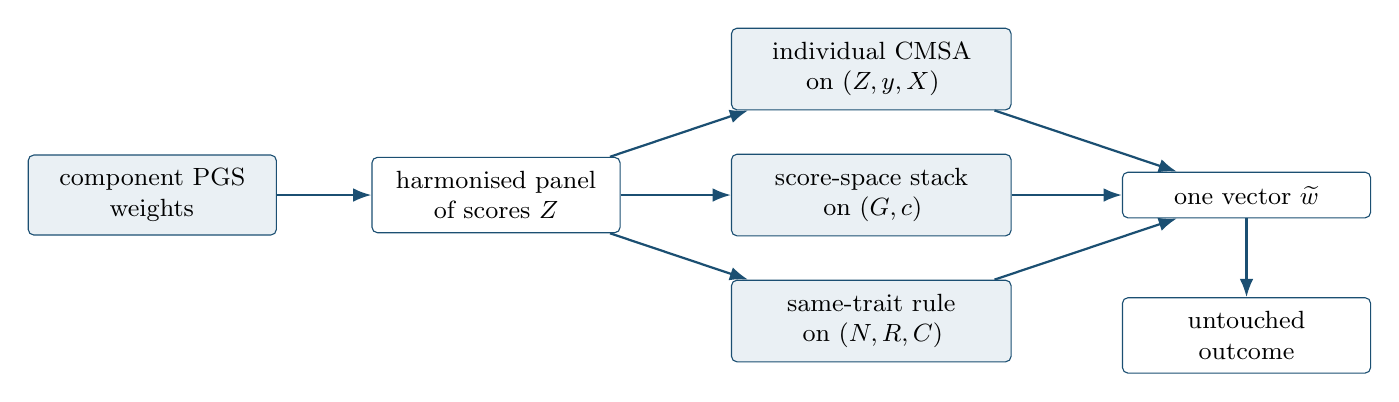
\begin{tikzpicture}[
  font=\small,
  box/.style={draw=ink,rounded corners=2pt,align=center,
              inner sep=5pt,fill=white,text width=28mm},
  source/.style={box,fill=soft},
  method/.style={box,fill=soft,text width=32mm},
  arr/.style={-{Latex},ink,thick}
]
  \node[source] (weights) {component PGS\\weights};
  \node[box,right=12mm of weights] (panel)
    {harmonised panel\\of scores \(Z\)};
  \node[method,right=14mm of panel,yshift=16mm] (ind)
    {individual CMSA\\on \((Z,y,X)\)};
  \node[method,right=14mm of panel] (sum)
    {score-space stack\\on \((G,c)\)};
  \node[method,right=14mm of panel,yshift=-16mm] (meta)
    {same-trait rule\\on \((N,R,C)\)};
  \node[box,right=14mm of sum] (deploy)
    {one vector \(\widetilde w\)};
  \node[box,below=10mm of deploy] (eval)
    {untouched\\outcome};
  \draw[arr] (weights) -- (panel);
  \draw[arr] (panel) -- (ind);
  \draw[arr] (panel) -- (sum);
  \draw[arr] (panel) -- (meta);
  \draw[arr] (ind) -- (deploy);
  \draw[arr] (sum) -- (deploy);
  \draw[arr] (meta) -- (deploy);
  \draw[arr] (deploy) -- (eval);
\end{tikzpicture}}
\caption{One deployable score, three information routes. The
  routes are not interchangeable. Assessment data must be
  untouched by component discovery, combination fitting, and
  tuning.}
\label{fig:overview}
\end{figure}

%----------------------------------------------------------------------
\section{Selection index}
\label{sec:index}

A useful working model writes each standardised component score
as
\begin{equation}
  Z_k=R_k g_k+\sqrt{1-R_k^2}\,\varepsilon_k,
  \label{eq:score-model}
\end{equation}
where \(\Var(\varepsilon_k)=1\), every \(\varepsilon_k\) is
orthogonal to every genetic value in the model, and the residual
errors may be correlated across scores. The last orthogonality
condition is a mediation and transport assumption; the algebraic
decomposition of \(Z_k\) with respect to \(g_k\) alone does not
imply it.

Under independent residual errors,
\begin{equation}
  \rho_k=R_k r_G(k,f),
  \qquad
  C_{k\ell}=
  \begin{cases}
    1, & k=\ell,\\
    R_kR_\ell r_G(k,\ell), & k\ne\ell .
  \end{cases}
  \label{eq:rho-c}
\end{equation}
Discovery sample overlap is one mechanism that can correlate the
residuals. Shared pipelines, LD references, model fitting, and
other common estimation artifacts can do so as well. Conversely,
overlap need not induce a large covariance in every design.

For a weight vector \(w\), the squared genetic-value correlation
of the linear index is
\begin{equation}
  R^2(w)=\frac{(w^{\mathsf T}\rho)^2}{w^{\mathsf T}Cw}.
  \label{eq:index-r2}
\end{equation}
When \(C\) is positive definite, Cauchy--Schwarz gives
\begin{equation}
  w_\star \propto C^{-1}\rho,
  \qquad
  R^2_{\max}=\rho^{\mathsf T}C^{-1}\rho .
  \label{eq:index-optimum}
\end{equation}
This is the classical selection-index solution
\cite{smith1936,hazel1943}. The same algebra combines correlated
forecasts \cite{bates1969}. A pseudoinverse or ridge is needed
when \(C\) is singular. Neither repairs a misspecified \(\rho\).

\paragraph{Closed-form gain from one auxiliary trait.}
For the focal score and one auxiliary score with genetic
correlation \(r\), the exact increment above the focal score is
\begin{equation}
  \Delta R^2=
  \frac{r^2R_k^2(1-R_f^2)^2}
       {1-r^2R_f^2R_k^2}.
  \label{eq:two-score-gain}
\end{equation}
Three factors are visible: squared genetic correlation, squared
auxiliary accuracy, and the squared information still missing
from the focal score. A large auxiliary GWAS cannot compensate
for genetic irrelevance, and a well-powered focal score leaves
less room to gain.

The Daetwyler reference model relates genetic-value accuracy to
GWAS power \cite{daetwyler2008},
\begin{equation}
  R_k^2=\frac{x_k}{1+x_k},
  \qquad
  x_k=\frac{N_k h_k^2}{M}.
  \label{eq:daetwyler}
\end{equation}
It is an upper-reference model under strong architecture and
population assumptions, not a per-score truth oracle. The
numerator of \eqref{eq:two-score-gain} then carries
\((1+x_f)^{-2}\): the absolute gain falls as the square of the
focal GWAS's own power. Table~\ref{tab:gain} records the
arithmetic at \(r_G=0.5\) and auxiliary \(R_k^2=0.5\).
Figure~\ref{fig:gain} plots the same equation against focal
sample size. Both displays are equation evaluations, not
empirical performance claims. The same asymmetry is long
established in multivariate genomic prediction: gains
concentrate on the underpowered trait when a correlated,
better-measured trait is available \cite{jia2012}. It is also
the shape of the published Multi-PGS result, whose largest
relative increase landed on ADHD \cite{albinana2023}.

\begin{table}[ht]
\centering
\caption{Exact two-score genetic-value increment from
  \eqref{eq:two-score-gain} under \eqref{eq:daetwyler}, with
  \(r_G=0.5\), auxiliary \(R_k^2=0.5\), \(h_f^2=0.2\), and
  \(M=20{,}000\), so \(x_f=N_f/100{,}000\). Phenotypic
  increments are these values times \(h_f^2\). The relative
  column is unaffected by that scaling.}
\label{tab:gain}
\small
\begin{tabular}{@{}rrrrr@{}}
\toprule
\(N_f\) & \(x_f\) & \(R_f^2\) alone & \(\Delta R^2\) &
relative gain \\
\midrule
\(10{,}000\) & \(0.1\) & \(0.091\) & \(0.104\) & \(+115\%\) \\
\(100{,}000\) & \(1\) & \(0.500\) & \(0.033\) & \(+6.7\%\) \\
\(400{,}000\) & \(4\) & \(0.800\) & \(0.006\) & \(+0.7\%\) \\
\(1{,}000{,}000\) & \(10\) & \(0.909\) & \(0.001\) & \(+0.1\%\) \\
\bottomrule
\end{tabular}
\end{table}

\begin{figure}[ht]
\centering
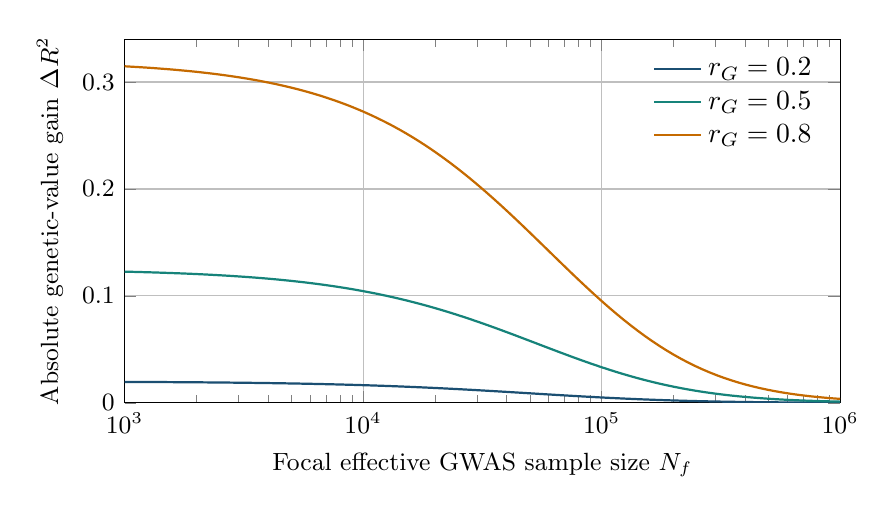
\begin{tikzpicture}
\begin{axis}[
  width=0.88\linewidth,height=62mm,
  xmode=log, xmin=1000,xmax=1000000,
  ymin=0,ymax=0.34,
  xlabel={Focal effective GWAS sample size \(N_f\)},
  ylabel={Absolute genetic-value gain \(\Delta R^2\)},
  grid=major,
  legend style={draw=none,fill=none,at={(0.98,0.98)},anchor=north east},
  tick label style={font=\small},
  label style={font=\small}
]
\addplot[ink,thick,domain=1000:1000000,samples=100]
 {(0.04*0.5*(1/(1+x/100000))^2)/
  (1-0.04*0.5*(x/100000)/(1+x/100000))};
\addlegendentry{\(r_G=0.2\)}
\addplot[teal,thick,domain=1000:1000000,samples=100]
 {(0.25*0.5*(1/(1+x/100000))^2)/
  (1-0.25*0.5*(x/100000)/(1+x/100000))};
\addlegendentry{\(r_G=0.5\)}
\addplot[amber,thick,domain=1000:1000000,samples=100]
 {(0.64*0.5*(1/(1+x/100000))^2)/
  (1-0.64*0.5*(x/100000)/(1+x/100000))};
\addlegendentry{\(r_G=0.8\)}
\end{axis}
\end{tikzpicture}
\caption{Analytical two-score gain from \eqref{eq:two-score-gain}.
The illustration fixes \(h_f^2=0.2\), \(M=20{,}000\), and
auxiliary \(R_k^2=0.5\), so \(x_f=N_f/100{,}000\). It is an
equation plot, not an empirical performance claim.}
\label{fig:gain}
\end{figure}

\FloatBarrier

%----------------------------------------------------------------------
\section{Three information routes}
\label{sec:routes}

Table~\ref{tab:routes} states the information contract. The
choice among routes is determined by the data that exist, not by
a single ranking of methods.

\begin{table}[ht]
\centering
\caption{Information and validation contract for the three
  combination routes.}
\label{tab:routes}
\scriptsize
\begin{tabularx}{\linewidth}{@{}L{26mm}Y Y Y@{}}
\toprule
\textbf{Route} & \textbf{Learns from} & \textbf{Selection / tuning} &
\textbf{Valid assessment} \\
\midrule
\code{multi\_pgs\_fit} & Individual score matrix, target
phenotype, optional covariates & Inner CMSA choices inside outer
folds; final coefficients average fold-selected fits; nested
heuristic may return the baseline &
Independent individuals who trained neither component scores nor
the combination \\
\code{multi\_pgs\_sumstats} & Target-GWAS cross-moments plus
external LD score Gram & Same moments, an independent second
GWAS, or PUMAS-style pseudo-splits & A third untouched GWAS or
independent individual-level cohort; tuning performance is not
assessment \\
\code{meta\_pgs} & Same-trait scores plus effective sample sizes
or expected accuracies; target score correlations for
decorrelation & No fitted tuning; ridge only stabilises inversion
& Independent target outcomes; simple metadata-derived weights
remain hypotheses until tested \\
\bottomrule
\end{tabularx}
\end{table}

\subsection{Individual-level penalised stacking}
\label{sec:individual}

Within each training fold, score columns are imputed and
standardised from that fold alone. With unpenalised covariates
\(X\), write \(\eta_i=b_0+X_i^{\mathsf T}\gamma+Z_i^{\mathsf T}\theta\).
The Gaussian or binomial elastic-net objective is
\begin{equation}
  \min_{b_0,\gamma,\theta}
  \mathcal Q(y,\eta)
  +\lambda\sum_{k=1}^{K}p_k
  \Bigl\{\alpha|\theta_k|
  +\tfrac{1-\alpha}{2}\theta_k^2\Bigr\},
  \label{eq:individual-objective}
\end{equation}
where
\begin{equation}
  \mathcal Q(y,\eta)
  =
  \begin{cases}
    (2n)^{-1}\sum_i(y_i-\eta_i)^2,
      & \text{Gaussian},\\
    -n^{-1}\sum_i\{y_i\eta_i-\log(1+\exp\eta_i)\},
      & \text{binomial}.
  \end{cases}
  \label{eq:loss}
\end{equation}
Covariates receive penalty factor zero. The Gaussian path uses
covariance updates; the binomial path uses IRLS with coordinate
descent \cite{friedman2010,zou2005}. For a standardised Gaussian
column with current partial score \(z_k^\star\), the coordinate
update is
\begin{equation}
  \theta_k \leftarrow
  \frac{\operatorname{sign}(z_k^\star)
        (|z_k^\star|-\lambda\alpha p_k)_+}
       {G_{kk}+\lambda(1-\alpha)p_k}.
  \label{eq:coordinate-update}
\end{equation}
In the Gaussian case, unpenalised covariate columns are
equivalent to residualising first (Frisch--Waugh--Lovell). The
equivalence does not hold for the binomial loss, where the IRLS
weights depend on the current fit.

CMSA fits a path inside folds, selects a fold-specific model,
and averages the selected coefficient vectors \cite{prive2019}.
Averaging is a variance reduction for an unstable selector: with
correlated scores and an \(\ell_1\) penalty, which of a set of
near-duplicates is picked is close to arbitrary. The averaged
support is the union of fold supports. Consequently
\code{selected()} reports predictive weights, not causal traits,
unique genetic contributors, or stable feature-selection
discoveries.

The package adds a nested outer-fold decision rule that falls
back to the unpenalised baseline when the apparent increment is
insufficient. Choosing a tuning parameter and assessing
performance are different tasks
\cite{stone1974,varma2006}. An ordinary CMSA validation fold
cannot also assess the stack: its phenotype selected that fold's
\((\alpha,\lambda)\). The nested estimate \(\mathrm{cv}\text{-}R^2\)
is a predictive loss gain of the inner stack over the explicit
unpenalised baseline on untouched outer rows. It is not the
OLS-recalibrated incremental \Rtwo{} of
\S\ref{sec:deploy}. The one-standard-error fallback fed by this
estimate is a deployment heuristic, not a hypothesis test. In
the committed null benchmark, pure noise passed in
\ReportNullPasses{} of \ReportNullReplicates{} checked runs.

\subsection{Summary-statistic score-space stacking}
\label{sec:sumstat}

Let \(W_{\mathrm{LD}}\) contain component weights on the LD
source's standardised-genotype scale, \(D\) be its LD
correlation matrix, and \(W_{\mathrm{GWAS}}\) contain the same
component scores on the GWAS source's standardised-genotype
scale. The sufficient moments are
\begin{equation}
  G_{\mathrm{raw}}=
    W_{\mathrm{LD}}^{\mathsf T} D W_{\mathrm{LD}},
  \qquad
  c_{\mathrm{raw}}=
    W_{\mathrm{GWAS}}^{\mathsf T}z .
  \label{eq:score-moments}
\end{equation}
Writing \(A=\operatorname{diag}
(\sqrt{\operatorname{diag}(G_{\mathrm{raw}})})\), the fitted
coordinates use
\begin{equation}
  G=A^{-1}G_{\mathrm{raw}}A^{-1},
  \qquad
  c=A^{-1}c_{\mathrm{raw}} .
  \label{eq:standardized-moments}
\end{equation}
This is the same Gaussian objective as
\eqref{eq:individual-objective}, but in the span of the supplied
scores. At \(\alpha=1\), the lasso selects entire component
scores. It is inspired by the SNP-level lassosum quadratic
\cite{mak2017}, but it is not SNP-level lassosum: the fitted
variant effects cannot leave that span.

For a fixed coefficient vector, summary tuning evaluates
\begin{equation}
  \operatorname{MSE}(\theta)
    =\operatorname{var}(y)-2\theta^{\mathsf T}c
      +\theta^{\mathsf T}G\theta,
  \qquad
  \widetilde R^2(\theta)
    =\frac{(\theta^{\mathsf T}c)^2}
    {\operatorname{var}(y)\,\theta^{\mathsf T}G\theta}.
  \label{eq:summary-metrics}
\end{equation}
MSE, not squared correlation, selects the path because \Rtwo{}
is blind to a reversed predictor. An independent second GWAS can
tune the path; a third is still needed for assessment.
PUMAS-style pseudo-splitting uses a joint-Gaussian/CLT
covariance approximation \cite{zhao2021}. In the committed
calibration, relative covariance error is
\ReportPumasGaussianErrorPct\% for Gaussian and
\ReportPumasBinaryErrorPct\% for binary simulations. That
quantifies the approximation. It does not validate
pseudotuning as assessment. Every scalar and pseudo-split path
carries coordinate-descent status; iteration-exhausted
candidates are excluded rather than silently selected.

When \(D\) and \(z\) come from the same individuals, \(G\) and
\(c\) are exact sample moments. With an external LD reference
they are plug-in estimates. Sampling noise can put \(c\) outside
the range of \(G\), or make the plug-in \Rtwo{} exceed one.
Those are diagnostics, not automatic proof of bad data.

\subsection{Training-free same-trait combination}
\label{sec:meta}

The simple rules standardise component scores and use
\begin{equation}
  w_k\propto\sqrt{N_{\mathrm{eff},k}}
  \quad\text{or}\quad
  w_k\propto\sqrt{\widehat R_k^2}.
  \label{eq:meta-simple}
\end{equation}
The first is a power-limited approximation sourced from pipeline
code, not from the Hansen et al.\ preprint \cite{hansen2026}.
Under independent estimation errors, the exact same-trait GLS
direction is
\begin{equation}
  w_k\propto\frac{R_k}{1-R_k^2},
  \label{eq:meta-gls}
\end{equation}
so direct accuracy weighting is accurate only as every \(R_k\)
approaches zero. Accuracy saturates; the optimal weight does
not. Weighting by accuracy therefore under-weights a
well-powered GWAS more than weighting by sample size does.

The decorrelated rule is
\begin{equation}
  w_\delta\propto(C+\delta I)^{-1}\rho.
  \label{eq:meta-decorrelated}
\end{equation}
Its algebra is exact under \eqref{eq:index-optimum}, but small
error in \(\rho\) is amplified along low-eigenvalue directions
of \(C\). Ridge reduces that amplification only by moving the
result back toward an undecorrelated weighted sum. The
implemented \(\rho\) is a nonnegative magnitude. Every component
must first be oriented to the same positive target direction;
the rule cannot represent a genuinely negative target
correlation. If only Daetwyler proxies are available, the
checked real CAD diagnostic supports \code{expected\_r2}, not
\code{decorrelated}.

The same-trait assumption \(r_G(k,\ell)\approx 1\) is assumed,
not known. Nominally identical phenotype GWAS can have
\(r_G<1\) when definitions or ascertainment differ. Applied to
genuinely different traits the assumption is wrong, and a
learned combination is the right tool.

%----------------------------------------------------------------------
\section{Deployment and evaluation}
\label{sec:deploy}

Catalog scoring files are aligned by
\texttt{panel\allowbreak\_from\allowbreak\_catalog}.
Summary-statistic components are built by
\texttt{panel\allowbreak\_from\allowbreak\_sumstats} through
ldpred3 \cite{prive2020}. Identifier order, genome build, effect
orientation, and source-specific dosage standard deviation are
part of the statistical contract, not file-format trivia.

Write component \(k\)'s term as \(c_{jk}(g_j-\mu_{jk})\), with
\(c_{jk}=w_{jk}/\sigma_{jk}\) for a standardized score and
\(c_{jk}=w_{jk}\) for a raw score. Define
\(C_j=\sum_k\beta_k c_{jk}\) and
\(M_j=\sum_k\beta_k c_{jk}\mu_{jk}\). The exact one-row frozen
representation has
\begin{equation}
  \mu_j^\star=\frac{M_j}{C_j},\qquad
  \widetilde w_j=\sigma_j^\star C_j .
  \label{eq:frozen-weights}
\end{equation}
Raw allele-count components use the target mean and leave one
removable intercept. If \(C_j=0,M_j\ne0\), or
\(\mu_j^\star\notin[0,2]\), no valid single LDpred3 row can
preserve both observed dosage and reference-mean missing
imputation, so deployment is refused rather than silently
rescaled.

The frozen scoring scale should be carried to new cohorts.
Re-standardising each cohort independently can change
coefficients, calibration, and even the meaning of a fixed
threshold.

With covariates, the package reports the unnormalised increment
\begin{equation}
  R^2_{\mathrm{incremental}}
  =R^2_{\mathrm{covariates+score}}-R^2_{\mathrm{covariates}}.
  \label{eq:incremental-r2}
\end{equation}
The Albi\~nana paper instead divides this difference by
\(1-R^2_{\mathrm{covariates}}\) \cite{albinana2023}. Absolute
values are therefore not identical even when relative
comparisons share covariates. Ancestry principal components
belong in that covariate set. Without them a score can predict
ancestry rather than disease \cite{wray2013}.

For binary outcomes, with population prevalence \(\pi\), sample
case fraction \(p_s\), threshold \(t=\Phi^{-1}(1-\pi)\), density
\(\varphi(t)\), and \(i=\varphi(t)/\pi\), the implemented Lee
transformation is
\begin{equation}
  C_{\mathrm{LT}}=
  \frac{[\pi(1-\pi)]^2}{\varphi(t)^2p_s(1-p_s)},
  \quad
  \vartheta=
  \frac{i(p_s-\pi)}{1-\pi}
  \left\{\frac{i(p_s-\pi)}{1-\pi}-t\right\},
  \quad
  R_L^2=
  \frac{C_{\mathrm{LT}}R_O^2}
       {1+C_{\mathrm{LT}}\vartheta R_O^2}.
  \label{eq:liability-r2}
\end{equation}
This metric depends on a stated prevalence assumption
\cite{lee2012}. Observed-scale \Rtwo{} is not comparable across
ascertainment schemes.

Squared correlation hides sign reversal. Report signed
correlation, or at least verify its sign, alongside \Rtwo{}.
Neither a weighted sum nor a high \Rtwo{} is a calibrated
absolute risk.

%----------------------------------------------------------------------
\section{Simulation evidence}
\label{sec:evidence}

The validation evidence is organised into four levels that are
not pooled:
\begin{enumerate}
  \item algebraic identities and numerical invariants;
  \item unit and contract tests (\S\ref{sec:tests});
  \item replicated synthetic or real-LD simulations with checked
    raw rows;
  \item descriptive real-data diagnostics without an untouched
    outcome truth.
\end{enumerate}
A passing simulation establishes behaviour under that
simulation. It does not establish biological transport or
clinical benefit. Headline numbers below are derived from the
committed CSVs named in each caption; Appendix~\ref{app:repro}
records the digest.

\subsection{Individual stacking as an estimator}
\label{sec:fit}

Figure~\ref{fig:fit-accuracy} reports mean held-out \Rtwo{} over
30 seeds in each of eight regimes. Because the simulated genetic
value lies in the score span, this is an estimator sanity check,
not evidence of clinical efficacy.

\begin{figure}[ht]
\centering
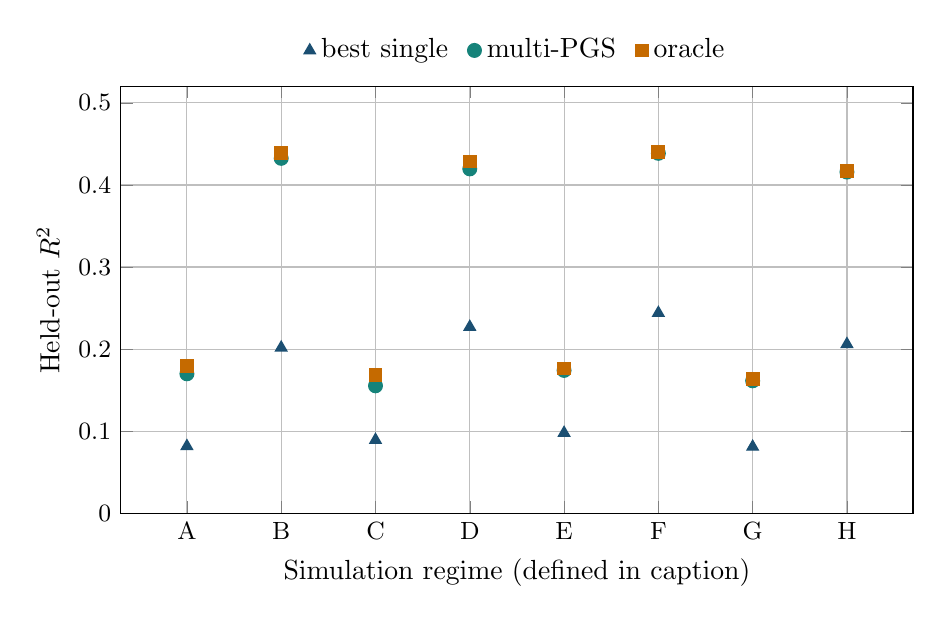
\begin{tikzpicture}
\begin{axis}[
  width=0.96\linewidth,height=70mm,
  symbolic x coords={A,B,C,D,E,F,G,H},
  xtick=data,
  ymin=0,ymax=0.52,
  ylabel={Held-out \(R^2\)},
  xlabel={Simulation regime (defined in caption)},
  grid=major,
  legend columns=3,
  legend style={draw=none,fill=none,at={(0.5,1.03)},anchor=south,
                /tikz/every even column/.append style={column sep=5pt}},
  tick label style={font=\small}
]
\addplot[only marks,mark=triangle*,mark size=2.4pt,ink]
 coordinates {(A,0.08169)(B,0.20177)(C,0.08925)(D,0.22703)
              (E,0.09785)(F,0.24406)(G,0.08094)(H,0.20603)};
\addlegendentry{best single}
\addplot[only marks,mark=*,mark size=2.5pt,teal]
 coordinates {(A,0.16985)(B,0.43249)(C,0.15522)(D,0.41961)
              (E,0.17398)(F,0.43857)(G,0.16131)(H,0.41576)};
\addlegendentry{multi-PGS}
\addplot[only marks,mark=square*,mark size=2.3pt,amber]
 coordinates {(A,0.17969)(B,0.43867)(C,0.16839)(D,0.42870)
              (E,0.17629)(F,0.44016)(G,0.16400)(H,0.41743)};
\addlegendentry{oracle}
\end{axis}
\end{tikzpicture}
\caption{Mean held-out \Rtwo{} over 30 seeds from
\protect\path{benchmarks/results/fit_accuracy_summary.csv}.
Regimes A--D use \(n=2000\), E--H use \(n=10{,}000\); A,B,E,F
use \(K=50\), the others \(K=200\); A,C,E,G use \(h^2=0.2\),
the others \(h^2=0.5\). The multi-PGS beats the
training-selected best single score in \ReportFitWins{} of
\ReportFitReplicates{} raw replicates. Because the simulated
genetic value lies in the score span, this is an estimator
sanity check, not evidence of clinical efficacy.}
\label{fig:fit-accuracy}
\end{figure}

Across the eight regimes, mean uplift over the selected single
score ranges from \ReportFitUpliftMin{} to \ReportFitUpliftMax{}
\Rtwo{}. Based on regime means, the fitted stack closes
\ReportFitGapClosedMinPct\%--\ReportFitGapClosedMaxPct\% of the
gap between the selected single score and the oracle. The
overall mean nested-CV minus held-out difference is
\(\ReportFitCvMinusHoldout\), slightly conservative in this
simulation. Support recall is high (\(0.84\)--\(1.00\) by
regime) while precision is only \(0.09\)--\(0.20\): the
averaged union support overstates sparsity, as the CMSA
construction predicts.

\subsection{Score-space identity and LD-reference sensitivity}
\label{sec:ld}

With exact individual moments, the summary and individual
standardised coefficients correlate
\ReportSumstatBetaCorrelation{} on average, and all compared
held-out \Rtwo{} values lie between \ReportSumstatRtwoMin{} and
\ReportSumstatRtwoMax. This supports the score-space identity
under the benchmark's strong-signal, small-\(K\) design.

Figure~\ref{fig:ld-reference} replaces the exact Gram by a
real-LD reference of finite size. At reference \(n=50\), true
fitted \Rtwo{} falls by \ReportLdTrueDropNfifty{} relative to
the infinite-reference result, while the own-reference estimate
is inflated by \ReportLdInflationNfifty{}
(\ReportLdInflationNfiftyPct\% of true fitted \Rtwo{}).
Reporting bias is larger than the loss in the fitted predictor.

\begin{figure}[ht]
\centering
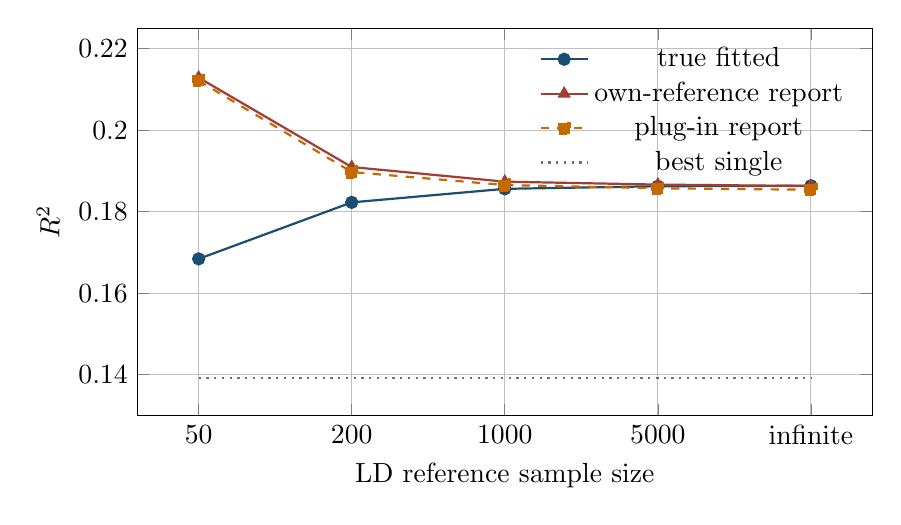
\begin{tikzpicture}
\begin{axis}[
  width=0.90\linewidth,height=65mm,
  symbolic x coords={50,200,1000,5000,infinite},
  xtick=data,
  ymin=0.13,ymax=0.225,
  xlabel={LD reference sample size},
  ylabel={\(R^2\)},
  grid=major,
  legend style={draw=none,fill=none,at={(0.98,0.98)},anchor=north east}
]
\addplot[ink,thick,mark=*]
 coordinates {(50,0.16842)(200,0.18228)(1000,0.18560)
              (5000,0.18624)(infinite,0.18636)};
\addlegendentry{true fitted}
\addplot[crit,thick,mark=triangle*]
 coordinates {(50,0.21288)(200,0.19095)(1000,0.18736)
              (5000,0.18664)(infinite,0.18629)};
\addlegendentry{own-reference report}
\addplot[amber,dashed,thick,mark=square*]
 coordinates {(50,0.21212)(200,0.18972)(1000,0.18653)
              (5000,0.18574)(infinite,0.18538)};
\addlegendentry{plug-in report}
\addplot[mid,dotted,thick]
 coordinates {(50,0.13918)(200,0.13918)(1000,0.13918)
              (5000,0.13918)(infinite,0.13918)};
\addlegendentry{best single}
\end{axis}
\end{tikzpicture}
\caption{Real-LD simulation from
\protect\path{real_ld_simulation_summary.csv}. At reference
\(n=50\), true fitted \Rtwo{} falls by \ReportLdTrueDropNfifty{}
relative to the infinite-reference result, while the
own-reference estimate is inflated by \ReportLdInflationNfifty{}
(\ReportLdInflationNfiftyPct\% of true fitted \Rtwo{}).
Reporting bias is larger than the loss in the fitted predictor.}
\label{fig:ld-reference}
\end{figure}

\subsection{Overlap inflation}
\label{sec:overlap}

Figure~\ref{fig:overlap} injects a known residual-error
correlation. True predictive \Rtwo{} barely moves. Reported
\Rtwo{} does. At overlap \(0.10\), reported-to-true \Rtwo{}
ratios are \ReportOverlapMultiRatioTen{} for multi-PGS and
\ReportOverlapSingleRatioTen{} for the single score; at
\(0.25\), they are \ReportOverlapMultiRatioTwentyFive{} and
\ReportOverlapSingleRatioTwentyFive. Cross-validation inside
the target cohort cannot remove discovery contamination shared
by every fold \cite{wray2013}.

Bivariate LDSC detected \ReportOverlapDetectedNonnull{} of
\ReportOverlapNonnullReplicates{} non-null runs and
\ReportOverlapDetectedNull{} of \ReportOverlapNullReplicates{}
null runs in this \(109{,}590\)-variant design. That does not
imply universal LDSC power. It refutes the absolute claim that
no downstream diagnostic can ever flag overlap. Exclusion by
design remains stronger than any post hoc test.

\begin{figure}[ht]
\centering
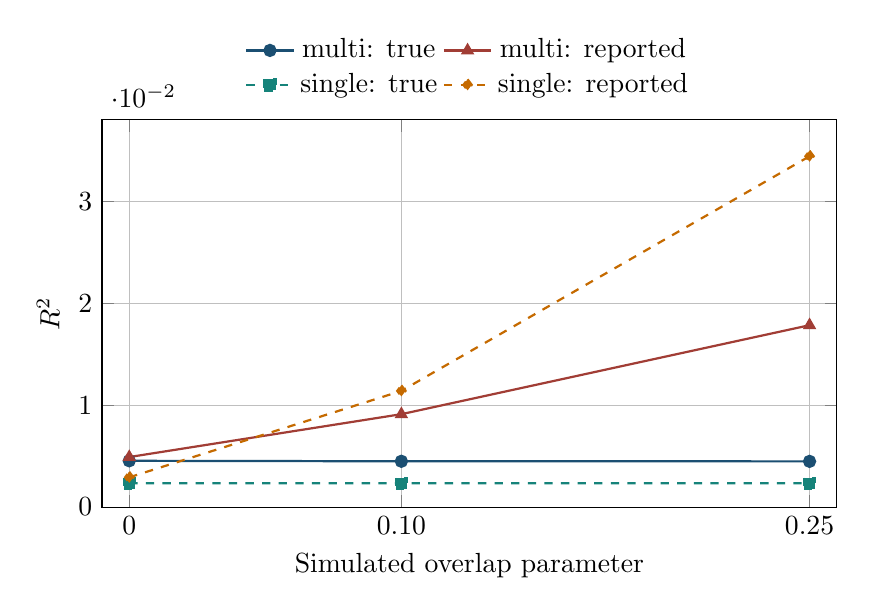
\begin{tikzpicture}
\begin{axis}[
  width=0.90\linewidth,height=65mm,
  xmin=-0.01,xmax=0.26,ymin=0,ymax=0.038,
  xtick={0,0.1,0.25},
  xticklabels={0,0.10,0.25},
  xlabel={Simulated overlap parameter},
  ylabel={\(R^2\)},
  grid=major,
  legend columns=2,
  legend style={draw=none,fill=none,at={(0.5,1.03)},anchor=south}
]
\addplot[ink,thick,mark=*]
 coordinates {(0,0.004539)(0.1,0.004493)(0.25,0.004484)};
\addlegendentry{multi: true}
\addplot[crit,thick,mark=triangle*]
 coordinates {(0,0.004909)(0.1,0.009115)(0.25,0.017845)};
\addlegendentry{multi: reported}
\addplot[teal,dashed,thick,mark=square*]
 coordinates {(0,0.002332)(0.1,0.002332)(0.25,0.002336)};
\addlegendentry{single: true}
\addplot[amber,dashed,thick,mark=diamond*]
 coordinates {(0,0.002917)(0.1,0.011397)(0.25,0.034424)};
\addlegendentry{single: reported}
\end{axis}
\end{tikzpicture}
\caption{Known-overlap simulation from
\protect\path{overlap_inflation_summary.csv}. At overlap 0.10,
reported-to-true \Rtwo{} ratios are
\ReportOverlapMultiRatioTen{} for multi-PGS and
\ReportOverlapSingleRatioTen{} for the single score; at 0.25,
they are \ReportOverlapMultiRatioTwentyFive{} and
\ReportOverlapSingleRatioTwentyFive. Bivariate LDSC detected
\ReportOverlapDetectedNonnull{} of
\ReportOverlapNonnullReplicates{} non-null runs and
\ReportOverlapDetectedNull{} of \ReportOverlapNullReplicates{}
null runs in this 109,590-variant design.}
\label{fig:overlap}
\end{figure}

\subsection{Decorrelation and proxy \(\rho\)}
\label{sec:decorr}

Figure~\ref{fig:decorrelation} contrasts two regimes. On the
left, the simulation supplies the intended accuracy structure:
the decorrelated rule holds its held-out \Rtwo{} as shared error
grows, while the simple rules decline. On the right, a single
checked 24-score CAD diagnostic replaces that \(\rho\) by
Daetwyler or sample-size proxies. Decorrelation then collapses.
The right panel is a contaminated regime-C score-space
description, not external outcome truth. The direct
expected-\Rtwo{} proxy is \ReportRealMetaExpectedRtwo, versus
\ReportRealMetaDecorrelatedRtwo{} after decorrelation.

Hence: the algebra of \eqref{eq:meta-decorrelated} is not a
licence to invert a poorly estimated \(\rho\). A well-estimated
\(C\) does not repair that.

\begin{figure}[ht]
\centering
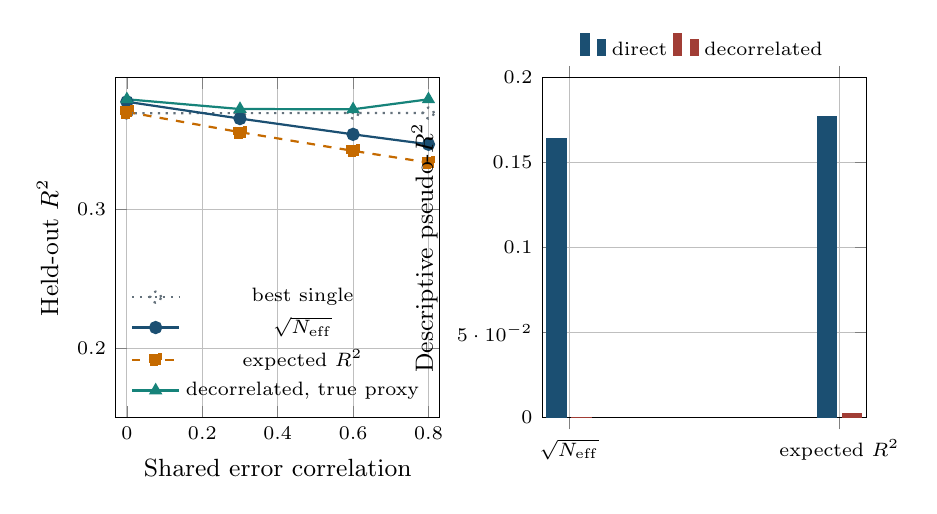
\begin{tikzpicture}
\begin{groupplot}[
  group style={group size=2 by 1,horizontal sep=13mm},
  width=0.47\linewidth,height=59mm,
  grid=major,
  tick label style={font=\scriptsize},
  label style={font=\small}
]
\nextgroupplot[
  xmin=-0.03,xmax=0.83,ymin=0.15,ymax=0.395,
  xlabel={Shared error correlation},
  ylabel={Held-out \(R^2\)},
  legend style={font=\scriptsize,draw=none,fill=none,at={(0.02,0.02)},
                anchor=south west}
]
\addplot[mid,dotted,thick,mark=o]
 coordinates {(0,0.36936)(0.3,0.36940)(0.6,0.36942)(0.8,0.36942)};
\addlegendentry{best single}
\addplot[ink,thick,mark=*]
 coordinates {(0,0.37758)(0.3,0.36547)(0.6,0.35411)(0.8,0.34693)};
\addlegendentry{\(\sqrt{N_{\rm eff}}\)}
\addplot[amber,dashed,thick,mark=square*]
 coordinates {(0,0.37024)(0.3,0.35567)(0.6,0.34221)(0.8,0.33379)};
\addlegendentry{expected \(R^2\)}
\addplot[teal,thick,mark=triangle*]
 coordinates {(0,0.37937)(0.3,0.37235)(0.6,0.37216)(0.8,0.37936)};
\addlegendentry{decorrelated, true proxy}

\nextgroupplot[
  ybar,bar width=7pt,
  symbolic x coords={sqrtN,expected},
  xtick=data,
  xticklabels={\(\sqrt{N_{\rm eff}}\),expected \(R^2\)},
  ymin=0,ymax=0.20,
  ylabel={Descriptive pseudo-\(R^2\)},
  legend style={font=\scriptsize,draw=none,fill=none,at={(0.5,1.02)},
                anchor=south,legend columns=2}
]
\addplot[fill=ink,draw=ink]
 coordinates {(sqrtN,0.16416)(expected,0.17729)};
\addlegendentry{direct}
\addplot[fill=crit,draw=crit]
 coordinates {(sqrtN,0.000167)(expected,0.002261)};
\addlegendentry{decorrelated}
\end{groupplot}
\end{tikzpicture}
\caption{Decorrelation behaves well when the simulation supplies
the intended accuracy structure (left, 30 seeds per point), but
collapses with proxy accuracies in the single checked 24-score
CAD diagnostic (right). The right panel is a contaminated
regime-C score-space description, not external outcome truth.
Sources: \protect\path{meta_rules_summary.csv} and
\protect\path{real_meta_rules_summary.csv}. The direct
expected-\Rtwo{} proxy is \ReportRealMetaExpectedRtwo, versus
\ReportRealMetaDecorrelatedRtwo{} after decorrelation.}
\label{fig:decorrelation}
\end{figure}

Table~\ref{tab:evidence} restates the headlines by evidence
level. The interpretations are part of the result.

\begin{table}[ht]
\centering
\caption{Headline validation evidence, separated by evidence
  level.}
\label{tab:evidence}
\scriptsize
\begin{tabularx}{\linewidth}{@{}L{31mm}L{34mm}Y@{}}
\toprule
\textbf{Artifact} & \textbf{Result} & \textbf{Interpretation} \\
\midrule
\path{fit_accuracy} & Multi-PGS wins
\ReportFitWins/\ReportFitReplicates{} held-out simulations;
uplift \ReportFitUpliftMin--\ReportFitUpliftMax{} &
Supports estimator sanity when truth lies in the score span;
does not establish real-outcome or clinical superiority. \\
\path{null_gate} & Noise passes
\ReportNullPasses/\ReportNullReplicates{} runs overall &
Shows the fallback is a decision heuristic, not a significance
test. \\
\path{sumstat_vs_individual} & coefficient correlation
\ReportSumstatBetaCorrelation; \Rtwo{}
\ReportSumstatRtwoMin--\ReportSumstatRtwoMax{} & Supports
exact-moment Gaussian equivalence in a small-\(K\),
strong-signal design. \\
\path{sumstat_calibration} & PUMAS covariance relative error
\ReportPumasGaussianErrorPct\% Gaussian,
\ReportPumasBinaryErrorPct\% binary &
Quantifies approximation error; it does not validate
pseudotuning as assessment. \\
\path{real_ld_simulation} & reference \(n=50\) report inflation
\ReportLdInflationNfifty{} &
Demonstrates reference-induced optimism under real LD. \\
\path{overlap_inflation} & up to
\ReportOverlapMultiRatioTwentyFive-fold multi-PGS and
\ReportOverlapSingleRatioTwentyFive-fold single-score inflation
& Demonstrates overlap danger under a known covariance
construction. \\
\path{real_meta_rules} & direct expected-\Rtwo{} proxy
\ReportRealMetaExpectedRtwo{} versus decorrelated
\ReportRealMetaDecorrelatedRtwo{} & Shows severe proxy
sensitivity in one regime-C CAD diagnostic; cannot rank methods
externally. \\
\bottomrule
\end{tabularx}
\end{table}

\FloatBarrier

%----------------------------------------------------------------------
\section{Unit tests and numerical contracts}
\label{sec:tests}

The complete automated suite passed \ReportTestCount{} of
\ReportTestCount{} tests in the environment of
Appendix~\ref{app:repro}. The contracts that carry the model,
rather than the plumbing, are these.

\paragraph{Algebra and scale.}
Standardisation and back-transformation, coordinate updates,
Gram ranges, projection identity and idempotence, and invariance
to a positive rescaling of a score.

\paragraph{Fitting contracts.}
Shape and scale validation, tuning separated from assessment,
frozen weights, convergence logs, deterministic seeds, and
baseline fallback. Gaussian unpenalised columns match an
explicit Frisch--Waugh--Lovell reference.

\paragraph{Genomic data handling.}
Allele orientation, ambiguous variants, duplicate handling,
LD/GWAS scale agreement, and missing-data behaviour.

\paragraph{Evaluation.}
Continuous and binary metrics, the Lee transformation, and
intervals that remain conditional on the supplied scores.

These tests pin the implementation to the mathematics in
\S\ref{sec:index}--\S\ref{sec:deploy}. They do not pin it to a
scientific claim about real GWAS.

\begin{table}[ht]
\centering
\caption{Automated verification layers and their interpretation.}
\label{tab:verification}
\small
\begin{tabularx}{\linewidth}{@{}L{34mm}Y L{37mm}@{}}
\toprule
\textbf{Layer} & \textbf{Representative assertions} &
\textbf{Result} \\
\midrule
Algebra and numerics & Standardisation and back-transformation,
coordinate updates, Gram ranges, projection identity and
idempotence, and score-rescaling invariance & Passed in the
full test suite \\
Fitting contracts & Shape and scale validation, tuning
separation, frozen weights, convergence logs, deterministic
seeds, and baseline fallback & Passed in the full test suite \\
Genomic data handling & Allele orientation, ambiguous variants,
duplicate handling, LD/GWAS scale agreement, and missing-data
behaviour & Passed in the full test suite \\
Evaluation and documentation & Continuous and binary metrics,
liability conversion, cited resources, benchmark result
consistency, and example paths & Passed in the full test suite \\
Distributions & Expected source and wheel contents, installed
import, and command-line smoke checks & Passed in the package
build checks \\
\bottomrule
\end{tabularx}
\end{table}

%----------------------------------------------------------------------
\section{Interpretation limits}
\label{sec:limits}

\begin{enumerate}
  \item \textbf{No causal interpretation.} Coefficients optimise
  prediction under correlation and penalisation. They do not
  estimate genetic correlations, mediation, or trait-specific
  causal contributions.
  \item \textbf{No automatic overlap cure.} Cross-validation
  inside a target cohort cannot remove discovery contamination
  shared by every fold. Bivariate LDSC or named-cohort metadata
  may flag overlap under favourable conditions. Exclusion by
  design is stronger.
  \item \textbf{No ancestry model.} Fitting weights in a target
  cohort does not repair discovery-score or LD-reference
  non-portability \cite{martin2019}. Absolute risk and score
  means are particularly unsafe across ancestries. Combining
  Catalog scores of many European-derived traits is not MIXPRS
  and does not substitute for a multi-population construction
  method \cite{xu2026}.
  \item \textbf{Direction matters.} Squared correlation hides
  sign reversal, and the training-free expected-\Rtwo{} routes
  assume consistent positive trait orientation.
  \item \textbf{No clinical calibration.} A high ranking metric
  is not a calibrated probability. Calibration intercept and
  slope, subgroup performance, decision utility, and an
  externally justified prevalence are separate requirements.
  \item \textbf{Conditional uncertainty.} The package bootstrap
  conditions on fixed component scores and their discovered
  weights. It does not propagate component-GWAS, LD-reference,
  or architecture-estimation uncertainty. Incremental \Rtwo{} is
  truncated at zero, so a null score produces a bootstrap
  interval whose lower end is \(0\) by construction.
\end{enumerate}

%----------------------------------------------------------------------
\section{Conclusion}
\label{sec:conclusion}

The central idea is ordinary. Move a difficult multi-trait
genomic problem into a smaller space of component scores, then
choose weights using the information that actually exists. The
selection-index derivation says when gains are possible. The
individual and summary Gaussian objectives say how weights are
learned. The same-trait rules are transparent constructions
whose accuracy assumptions must be checked externally.

That is not the MIXPRS problem. MIXPRS ensembles two
multi-population methods of one trait after data fission
\cite{xu2026}. This package stacks already-built scores,
typically of many traits, or combines same-trait GWAS by
metadata. The shared summary-statistic quadratic and PUMAS-style
split \cite{zhao2021,zhao2024} do not identify the estimands.

The choice among routes is an information problem, not a
universal ranking. Individual fitting is appropriate when a
target phenotype and honest resampling are available. Summary
fitting preserves the same score-space structure when GWAS
cross-moments and LD are available. Training-free rules remain
hypotheses until an untouched outcome is scored. For a
same-trait method-by-ancestry ensemble, use MIXPRS rather than
relabelling this package.

The committed tests and benchmarks demonstrate scale handling,
numerical equivalence, controlled prediction gains, null
behaviour, and sensitivity to LD-reference quality and
discovery overlap. They explain how the software behaves under
known conditions. They deliberately stop short of claiming
clinical validity, portability, or calibrated risk.

%----------------------------------------------------------------------
\appendix
\section{Reproducibility}
\label{app:repro}

Quantitative statements in \S\ref{sec:evidence} are generated
from committed CSVs by \texttt{generate\allowbreak\_evidence.py}.
The input SHA-256 is the freshness authority; the source
revision is generation context.

\begin{center}
\small
\begin{tabular}{@{}ll@{}}
\toprule
Package & \pkg{multipgs} \ReportPackageVersion \\
Source revision & \texttt{\ReportSourceRevision} \\
Input digest & \texttt{\ReportInputDigest} \\
Tests & \ReportTestCount{} passed \\
Runtime & Python \ReportPythonVersion, NumPy
\ReportNumpyVersion, scikit-learn \ReportScikitLearnVersion,
pytest \ReportPytestVersion, ldpred3 \ReportLdpredThreeVersion \\
\bottomrule
\end{tabular}
\end{center}

The named artifacts are
\path{fit_accuracy},
\path{null_gate},
\path{sumstat_vs_individual},
\path{sumstat_calibration},
\path{real_ld_simulation},
\path{overlap_inflation},
\path{meta_rules}, and
\path{real_meta_rules},
each with a checked summary and a provenance file under
\path{benchmarks/results/}.

\begin{thebibliography}{99}

\bibitem{smith1936}
H.~F. Smith.
\newblock A discriminant function for plant selection.
\newblock \emph{Annals of Eugenics}, 7(3):240--250, 1936.
\newblock \doi{10.1111/j.1469-1809.1936.tb02143.x}.

\bibitem{hazel1943}
L.~N. Hazel.
\newblock The genetic basis for constructing selection indexes.
\newblock \emph{Genetics}, 28(6):476--490, 1943.
\newblock \doi{10.1093/genetics/28.6.476}.

\bibitem{bates1969}
J.~M. Bates and C.~W.~J. Granger.
\newblock The combination of forecasts.
\newblock \emph{Operational Research Quarterly}, 20(4):451--468, 1969.
\newblock \doi{10.1057/jors.1969.103}.

\bibitem{stone1974}
M.~Stone.
\newblock Cross-validatory choice and assessment of statistical
predictions.
\newblock \emph{Journal of the Royal Statistical Society: Series~B},
36(2):111--133, 1974.
\newblock \doi{10.1111/j.2517-6161.1974.tb00994.x}.

\bibitem{zou2005}
H.~Zou and T.~Hastie.
\newblock Regularization and variable selection via the elastic net.
\newblock \emph{Journal of the Royal Statistical Society: Series~B},
67(2):301--320, 2005.
\newblock \doi{10.1111/j.1467-9868.2005.00503.x}.

\bibitem{varma2006}
S.~Varma and R.~Simon.
\newblock Bias in error estimation when using cross-validation for
model selection.
\newblock \emph{BMC Bioinformatics}, 7:91, 2006.
\newblock \doi{10.1186/1471-2105-7-91}.

\bibitem{daetwyler2008}
H.~D. Daetwyler, B.~Villanueva, and J.~A. Woolliams.
\newblock Accuracy of predicting the genetic risk of disease using a
genome-wide approach.
\newblock \emph{PLoS ONE}, 3(10):e3395, 2008.
\newblock \doi{10.1371/journal.pone.0003395}.

\bibitem{friedman2010}
J.~Friedman, T.~Hastie, and R.~Tibshirani.
\newblock Regularization paths for generalized linear models via
coordinate descent.
\newblock \emph{Journal of Statistical Software}, 33(1), 2010.
\newblock \doi{10.18637/jss.v033.i01}.

\bibitem{jia2012}
Y.~Jia and J.-L. Jannink.
\newblock Multiple-trait genomic selection methods increase genetic
value prediction accuracy.
\newblock \emph{Genetics}, 192(4):1513--1522, 2012.
\newblock \doi{10.1534/genetics.112.144246}.

\bibitem{lee2012}
S.~H. Lee, M.~E. Goddard, N.~R. Wray, and P.~M. Visscher.
\newblock A better coefficient of determination for genetic profile
analysis.
\newblock \emph{Genetic Epidemiology}, 36(3):214--224, 2012.
\newblock \doi{10.1002/gepi.21614}.

\bibitem{dudbridge2013}
F.~Dudbridge.
\newblock Power and predictive accuracy of polygenic risk scores.
\newblock \emph{PLOS Genetics}, 9(3):e1003348, 2013.
\newblock \doi{10.1371/journal.pgen.1003348}.

\bibitem{wray2013}
N.~R. Wray, J.~Yang, B.~J. Hayes, A.~L. Price, M.~E. Goddard, and
P.~M. Visscher.
\newblock Pitfalls of predicting complex traits from {SNP}s.
\newblock \emph{Nature Reviews Genetics}, 14(7):507--515, 2013.
\newblock \doi{10.1038/nrg3457}.

\bibitem{mak2017}
T.~S.~H. Mak, R.~M. Porsch, S.~W. Choi, X.~Zhou, and P.~C. Sham.
\newblock Polygenic scores via penalized regression on summary
statistics.
\newblock \emph{Genetic Epidemiology}, 41(6):469--480, 2017.
\newblock \doi{10.1002/gepi.22050}.

\bibitem{marquez2017}
C.~M\'arquez-Luna, P.-R. Loh, {SAT2D Consortium}, {SIGMA Type 2
Diabetes Consortium}, and A.~L. Price.
\newblock Multiethnic polygenic risk scores improve risk prediction
in diverse populations.
\newblock \emph{Genetic Epidemiology}, 41(8):811--823, 2017.
\newblock \doi{10.1002/gepi.22083}.

\bibitem{inouye2018}
M.~Inouye et~al.
\newblock Genomic risk prediction of coronary artery disease in
480{,}000 adults.
\newblock \emph{Journal of the American College of Cardiology},
72(16):1883--1893, 2018.
\newblock \doi{10.1016/j.jacc.2018.07.079}.

\bibitem{krapohl2018}
E.~Krapohl et~al.
\newblock Multi-polygenic score approach to trait prediction.
\newblock \emph{Molecular Psychiatry}, 23:1368--1374, 2018.
\newblock \doi{10.1038/mp.2017.163}.

\bibitem{maier2018}
R.~M. Maier et~al.
\newblock Improving genetic prediction by leveraging genetic
correlations among human diseases and traits.
\newblock \emph{Nature Communications}, 9:989, 2018.
\newblock \doi{10.1038/s41467-017-02769-6}.

\bibitem{turley2018}
P.~Turley et~al.
\newblock Multi-trait analysis of genome-wide association summary
statistics using {MTAG}.
\newblock \emph{Nature Genetics}, 50(2):229--237, 2018.
\newblock \doi{10.1038/s41588-017-0009-4}.

\bibitem{martin2019}
A.~R. Martin, M.~Kanai, Y.~Kamatani, Y.~Okada, B.~M. Neale, and
M.~J. Daly.
\newblock Clinical use of current polygenic risk scores may
exacerbate health disparities.
\newblock \emph{Nature Genetics}, 51(4):584--591, 2019.
\newblock \doi{10.1038/s41588-019-0379-x}.

\bibitem{prive2019}
F.~Priv\'e, H.~Aschard, and M.~G.~B. Blum.
\newblock Efficient implementation of penalized regression for
genetic risk prediction.
\newblock \emph{Genetics}, 212(1):65--74, 2019.
\newblock \doi{10.1534/genetics.119.302019}.

\bibitem{choi2020}
S.~W. Choi, T.~S.-H. Mak, and P.~F. O'Reilly.
\newblock Tutorial: a guide to performing polygenic risk score
analyses.
\newblock \emph{Nature Protocols}, 15:2759--2772, 2020.
\newblock \doi{10.1038/s41596-020-0353-1}.

\bibitem{prive2020}
F.~Priv\'e, J.~Arbel, and B.~J. Vilhj\'almsson.
\newblock {LDpred2}: better, faster, stronger.
\newblock \emph{Bioinformatics}, 36(22--23):5424--5431, 2020.
\newblock \doi{10.1093/bioinformatics/btaa1029}.

\bibitem{lambert2021}
S.~A. Lambert et~al.
\newblock The {P}olygenic {S}core {C}atalog as an open database for
reproducibility and systematic evaluation.
\newblock \emph{Nature Genetics}, 53(4):420--425, 2021.
\newblock \doi{10.1038/s41588-021-00783-5}.

\bibitem{zhao2021}
Z.~Zhao, Y.~Wu, J.~Miao, Y.~Song, X.~Zhong, et~al.
\newblock {PUMAS}: fine-tuning polygenic risk scores with {GWAS}
summary statistics.
\newblock \emph{Genome Biology}, 22:257, 2021.
\newblock \doi{10.1186/s13059-021-02479-9}.

\bibitem{zhao2024}
Z.~Zhao et~al.
\newblock Optimizing and benchmarking polygenic risk scores with
{GWAS} summary statistics.
\newblock \emph{Genome Biology}, 25:260, 2024.
\newblock \doi{10.1186/s13059-024-03400-w}.

\bibitem{albinana2023}
C.~Albi\~nana et~al.
\newblock Multi-{PGS} enhances polygenic prediction by combining
937 polygenic scores.
\newblock \emph{Nature Communications}, 14:4702, 2023.
\newblock \doi{10.1038/s41467-023-40330-w}.

\bibitem{truong2024}
B.~Truong et~al.
\newblock Integrative polygenic risk score improves the prediction
accuracy of complex traits and diseases.
\newblock \emph{Cell Genomics}, 4(4):100523, 2024.
\newblock \doi{10.1016/j.xgen.2024.100523}.

\bibitem{xu2026}
L.~Xu, Y.~Dong, X.~Zeng, Z.~Bian, G.~Zhou, L.~Guan, and
H.~Zhao.
\newblock {MIXPRS} enables multi-population and multi-method
polygenic risk scores using summary statistics.
\newblock \emph{Nature Genetics}, 58:1583--1594, 2026.
\newblock \doi{10.1038/s41588-026-02637-4}.

\bibitem{hansen2026}
O.~Hansen et~al.
\newblock Mapping genetic architecture of thousands of complex
traits using {GWAS} summary statistics.
\newblock Research Square (preprint, not peer reviewed), 2026.
\newblock \doi{10.21203/rs.3.rs-9415305/v1}.

\end{thebibliography}

\end{document}
